\documentclass[../template.tex]{subfiles}
\begin{document}
	\begin{center}
		\normalsize\bfseries\MakeUppercase{ВВЕДЕНИЕ}
	\end{center}
	\addcontentsline{toc}{section}{ВВЕДЕНИЕ}

	
\textbf{Цель данной работы} -- важная цель.

\textbf{Задачи:}
\begin{itemize}
	\item задачи под цель списком
\end{itemize}
	
\cite{kuchyanovLazernayaGeneraciyaOpalopodobnyh2016} % пример вставки цитаты

Вставка картинки. Смотри \refris{fig:sample_pic}

\begin{figure}[h]
	\centering
	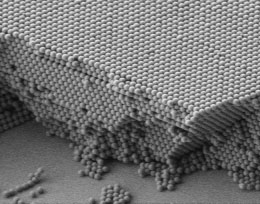
\includegraphics[width=0.5\linewidth]{../images/sample_pic.png}
	\caption{Sample pic}
	\label{fig:sample_pic}
\end{figure}

Вставка множества картинок (subfigure). Обращаться можно по всем ключам \refris{fig:subfig_a}, \refris{fig:subfig_b}, \refris{fig:fig_of_subfig}

\begin{figure}[h]
	\centering
	\begin{subfigure}[t]{.48\textwidth}
		\centering
		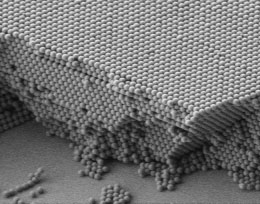
\includegraphics[height=.7\linewidth]{../images/sample_pic.png}  
		\caption{Энергетическая диаграмма электронов в полупроводнике}
		\label{fig:subfig_a}
	\end{subfigure}
	\hfill
	\begin{subfigure}[t]{.48\textwidth}
		\centering
		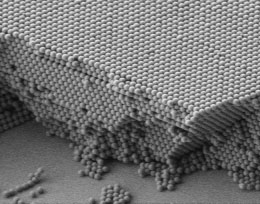
\includegraphics[height=.7\linewidth]{../images/sample_pic.png} 
		\caption{Энергетическая диаграмма фотонов в фотонном кристалле}
		\label{fig:subfig_b}
	\end{subfigure}
	\caption{Сравнение полупроводника и фотонного кристалла. Обращение к буквам \subref{fig:subfig_a} и \subref{fig:subfig_b}}
	\label{fig:fig_of_subfig}
\end{figure}	
	
	Пример создания таблицы см. \reftab{tab:summarized_d_D_l} oidjlahsdfk askjdfhaisjkdbfkajs dfkjasb d fnkas dfa  f s dg as df as df as df as df as df asd f asd f asdf 
	
	
	\begin{table}[h]
		\centering
		\begin{tabular}{|c|c|c|c|c|c|c|}
			\hline
			$d\rt{теор}$, нм & $D\rt{теор}$, нм & $\lambda\rt{теор}$, нм & $d\rt{эксп}$, нм & $D\rt{эксп}$, нм & $\lambda\rt{эксп}$, нм & $n\rt{эксп}$ \\ \hline
			252 & 300 & 668       & 244       & 299       & 689             & 1.410     \\ \hline
			325 & 388 & 864       & 325       & 398       & 863             & 1.32      \\ \hline
			289 & 347 & 773       & 283       & 347       & 774             & 1.364     \\ \hline
			224 & 267 & 595       & 220       & 269       & 611             & 1.39      \\ \hline
			317 & 384 & 855       & 324       & 397       & 857             & 1.32      \\ \hline
		\end{tabular}
		\caption{d -- диаметр сферы, D -- расстояние между сферами (1/0.86d), $\lambda$ -- ФЗЗ, n -- коэффициент преломления}
		\label{tab:summarized_d_D_l}
	\end{table}
	
	Пример нумерованных списков
	\begin{enumerate}
		\item \blindtext
		\item \blindtext
		\begin{enumerate}
			\item \blindtext
		\end{enumerate}
	\end{enumerate}
	
	Пример bullet списков
	\begin{itemize}
		\item \blindtext
		\item \blindtext
		\begin{itemize}
			\item \blindtext
		\end{itemize}
	\end{itemize}
	
\end{document}
